\let\negmedspace\undefined
\let\negthickspace\undefined
\documentclass{article}
\usepackage{cite}
\usepackage{amsmath,amssymb,amsfonts,amsthm}
\usepackage{algorithmic}
\usepackage{graphicx}
\usepackage{textcomp}
\usepackage{xcolor}
\usepackage{txfonts}
\usepackage{float}
\usepackage{listings}
\usepackage{enumitem}
\usepackage{mathtools}
\usepackage{gensymb}
\usepackage{tfrupee}
\usepackage[breaklinks=true]{hyperref}
\usepackage{tkz-euclide} % loads  TikZ and tkz-base
\usepackage{listings}
\usepackage{gvv}
%
%\usepackage{setspace}
%\usepackage{gensymb}
%\doublespacing
%\singlespacing

%\usepackage{graphicx}
%\usepackage{amssymb}
%\usepackage{relsize}
%\usepackage[cmex10]{amsmath}
%\usepackage{amsthm}
%\interdisplaylinepenalty=2500
%\savesymbol{iint}
%\usepackage{txfonts}
%\restoresymbol{TXF}{iint}
%\usepackage{wasysym}
%\usepackage{amsthm}
%\usepackage{iithtlc}
%\usepackage{mathrsfs}
%\usepackage{txfonts}
%\usepackage{stfloats}
%\usepackage{bm}
%\usepackage{cite}
%\usepackage{cases}
%\usepackage{subfig}
%\usepackage{xtab}
%\usepackage{longtable}
%\usepackage{multirow}
%\usepackage{algorithm}
%\usepackage{algpseudocode}
%\usepackage{enumitem}
%\usepackage{mathtools}
%\usepackage{tikz}
%\usepackage{circuitikz}
%\usepackage{verbatim}
%\usepackage{tfrupee}
%\usepackage{stmaryrd}
%\usetkzobj{all}
%    \usepackage{color}                                            %%
%    \usepackage{array}                                            %%
%    \usepackage{longtable}                                        %%
%    \usepackage{calc}                                             %%
%    \usepackage{multirow}                                         %%
%    \usepackage{hhline}                                           %%
%    \usepackage{ifthen}                                           %%
  %optionally (for landscape tables embedded in another document): %%
%    \usepackage{lscape}
%\usepackage{multicol}
%\usepackage{chngcntr}
%\usepackage{enumerate}

%\usepackage{wasysym}
%\documentclass[conference]{IEEEtran}
%\IEEEoverridecommandlockouts
% The preceding line is only needed to identify funding in the first footnote. If that is unneeded, please comment it out.

\newtheorem{theorem}{Theorem}[section]
\newtheorem{problem}{Problem}
\newtheorem{proposition}{Proposition}[section]
\newtheorem{lemma}{Lemma}[section]
\newtheorem{corollary}[theorem]{Corollary}
\newtheorem{example}{Example}[section]
\newtheorem{definition}[problem]{Definition}
%\newtheorem{thm}{Theorem}[section]
%\newtheorem{defn}[thm]{Definition}
%\newtheorem{algorithm}{Algorithm}[section]
%\newtheorem{cor}{Corollary}
\newcommand{\BEQA}{\begin{eqnarray}}
\newcommand{\EEQA}{\end{eqnarray}}
%\newcommand{\define}{\stackrel{\triangle}{=}}
\theoremstyle{remark}
\newtheorem{rem}{Remark}

%\bibliographystyle{ieeetr}
\begin{document}
\title{LATEX ASSIGNMENT}
\author{SHAIK MOHAMMAD SAHIL}
\date{23-09-2023}
\maketitle
\section*{CLASS 10} 
\subsection*{Circles}
\date{}
\maketitle
\begin{enumerate}[label=\arabic*.,ref=\theenumi]
    \item In \figref{fig:fig1.png}, $PQ\parallel BC$, $PQ=3cm$, $BC=9cm$  and $AC=7.5cm$. Find the length of $AQ$.
    \begin{figure}[H]
        \centering
        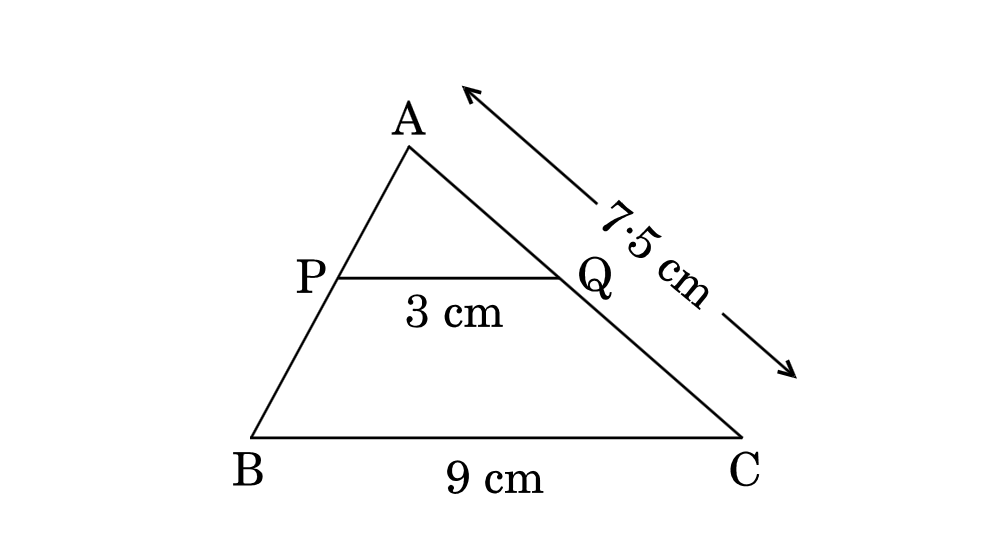
\includegraphics[width=\columnwidth]{./figs/figure1.png}
        \caption{$PQ\left |  \right | BC$}
        \label{fig:fig1.png}
    \end{figure}

    \item Draw a circle of radius $2.5cm$. Take a point $P$ outside the circle at a distance of $7cm$ from the centre. Then construct a pair of tangents to the circle from point $P$.

    \item Sides $AB$ and $AC$ and median $AD$ of $\triangle ABC$ are respectively proportional to sides $PQ$ and $PR$ and median $PM$ of $\triangle PQR$. Show that $\triangle ABC$  $\sim$  $\triangle PQR$.

     \item In \figref{fig:fig2.png} $BN$ and $CM$ are medians of a  $\triangle ABC$ right-angled at $A$. Prove that $4 (BN^2 + CM^2) = 5 BC^2$.

    \begin{figure}[H]
        \centering
        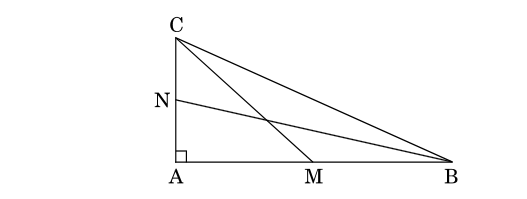
\includegraphics[width=\columnwidth]{./figs/figure2.png}
        \caption{ $BN$ and $CM$ are medians}
        \label{fig:fig2.png}
    \end{figure}

     \item Construct a pair of tangents to a circle of radius $4cm$ from a point $P$ lying outside the circle at a distance of $6cm$ from the centre.


     \item     

     \begin{enumerate}[label=(\alph*)]

     \item Draw a line segment $AB$ of length $8cm$ and locate a point $P$ 
      on $AB$ such that $AP$ : $PB$ = $1$ : $5$.

      \item  Draw a circle of radius $3 cm$. From a point $P$ lying outside the 
       circle at a distance of $6cm$ from its centre, construct two tangents
       $PA$ and $PB$ to the circle.

       \end{enumerate}

       \item Construct a pair of tangents to a circle of radius $5cm$ which are inclined each other at an angle of $60^{o}$.


        \item Write the steps of construction for constructing a pair of
         tangents to a circle of radius $4cm$ from a point $P$, at a distance
         of $7cm$ from its centre $O$.
   
\end{enumerate} 
\end{document}

